\documentclass{standalone}
\usepackage{tikz}
\begin{document}
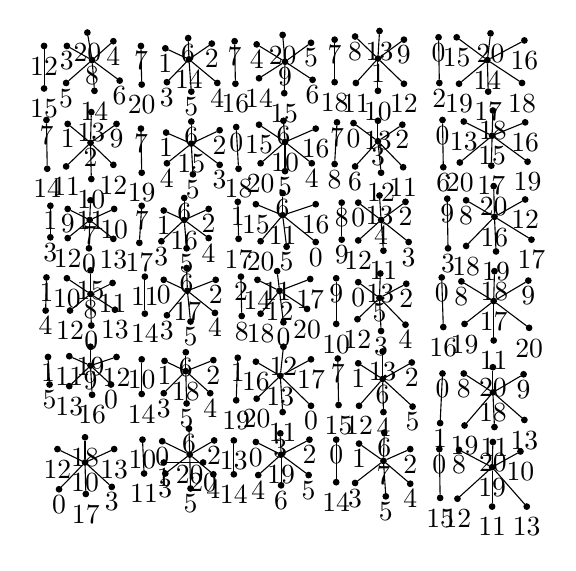
\begin{tikzpicture}[every node/.style={draw, circle, fill=black, minimum size=2pt, inner sep=0pt}]
\node[fill=black, label=below:{\color{black}$15$}] (G1N15) at (8.81,7.74) {};
\node[fill=black, label=below:{\color{black}$14$}] (G1N14) at (9.20,7.45) {};
\node[fill=black, label=below:{\color{black}$16$}] (G1N16) at (9.67,7.70) {};
\node[fill=black, label=below:{\color{black}$17$}] (G1N17) at (9.21,7.05) {};
\node[fill=black, label=below:{\color{black}$18$}] (G1N18) at (9.64,7.16) {};
\node[fill=black, label=below:{\color{black}$19$}] (G1N19) at (8.84,7.15) {};
\node[fill=black, label=below:{\color{black}$20$}] (G1N20) at (9.24,7.79) {};
\node[fill=black, label=below:{\color{black}$0$}] (G1N0) at (8.58,7.74) {};
\node[fill=black, label=below:{\color{black}$2$}] (G1N2) at (8.59,7.16) {};
\draw (G1N14) -- (G1N15);
\draw (G1N14) -- (G1N16);
\draw (G1N14) -- (G1N17);
\draw (G1N14) -- (G1N18);
\draw (G1N14) -- (G1N19);
\draw (G1N14) -- (G1N20);
\draw (G1N2) -- (G1N0);
\node[fill=black, label=below:{\color{black}$13$}] (G2N13) at (8.90,6.67) {};
\node[fill=black, label=below:{\color{black}$15$}] (G2N15) at (9.26,6.49) {};
\node[fill=black, label=below:{\color{black}$16$}] (G2N16) at (9.68,6.66) {};
\node[fill=black, label=below:{\color{black}$17$}] (G2N17) at (9.25,6.11) {};
\node[fill=black, label=below:{\color{black}$18$}] (G2N18) at (9.27,6.81) {};
\node[fill=black, label=below:{\color{black}$19$}] (G2N19) at (9.71,6.16) {};
\node[fill=black, label=below:{\color{black}$20$}] (G2N20) at (8.85,6.15) {};
\node[fill=black, label=below:{\color{black}$0$}] (G2N0) at (8.63,6.69) {};
\node[fill=black, label=below:{\color{black}$6$}] (G2N6) at (8.64,6.09) {};
\draw (G2N15) -- (G2N13);
\draw (G2N15) -- (G2N16);
\draw (G2N15) -- (G2N17);
\draw (G2N15) -- (G2N18);
\draw (G2N15) -- (G2N19);
\draw (G2N15) -- (G2N20);
\draw (G2N6) -- (G2N0);
\node[fill=black, label=below:{\color{black}$8$}] (G3N8) at (8.93,5.67) {};
\node[fill=black, label=below:{\color{black}$16$}] (G3N16) at (9.29,5.46) {};
\node[fill=black, label=below:{\color{black}$12$}] (G3N12) at (9.68,5.68) {};
\node[fill=black, label=below:{\color{black}$17$}] (G3N17) at (9.76,5.17) {};
\node[fill=black, label=below:{\color{black}$18$}] (G3N18) at (8.93,5.09) {};
\node[fill=black, label=below:{\color{black}$19$}] (G3N19) at (9.31,5.02) {};
\node[fill=black, label=below:{\color{black}$20$}] (G3N20) at (9.28,5.85) {};
\node[fill=black, label=below:{\color{black}$9$}] (G3N9) at (8.69,5.69) {};
\node[fill=black, label=below:{\color{black}$3$}] (G3N3) at (8.70,5.06) {};
\draw (G3N16) -- (G3N8);
\draw (G3N16) -- (G3N12);
\draw (G3N16) -- (G3N17);
\draw (G3N16) -- (G3N18);
\draw (G3N16) -- (G3N19);
\draw (G3N16) -- (G3N20);
\draw (G3N9) -- (G3N3);
\node[fill=black, label=below:{\color{black}$8$}] (G4N8) at (8.87,4.64) {};
\node[fill=black, label=below:{\color{black}$17$}] (G4N17) at (9.28,4.39) {};
\node[fill=black, label=below:{\color{black}$9$}] (G4N9) at (9.72,4.65) {};
\node[fill=black, label=below:{\color{black}$11$}] (G4N11) at (9.28,3.89) {};
\node[fill=black, label=below:{\color{black}$18$}] (G4N18) at (9.29,4.77) {};
\node[fill=black, label=below:{\color{black}$19$}] (G4N19) at (8.91,4.10) {};
\node[fill=black, label=below:{\color{black}$20$}] (G4N20) at (9.73,4.05) {};
\node[fill=black, label=below:{\color{black}$16$}] (G4N16) at (8.64,4.06) {};
\node[fill=black, label=below:{\color{black}$0$}] (G4N0) at (8.62,4.69) {};
\draw (G4N17) -- (G4N8);
\draw (G4N17) -- (G4N9);
\draw (G4N17) -- (G4N11);
\draw (G4N17) -- (G4N18);
\draw (G4N17) -- (G4N19);
\draw (G4N17) -- (G4N20);
\draw (G4N16) -- (G4N0);
\node[fill=black, label=below:{\color{black}$8$}] (G5N8) at (8.90,3.47) {};
\node[fill=black, label=below:{\color{black}$18$}] (G5N18) at (9.27,3.23) {};
\node[fill=black, label=below:{\color{black}$9$}] (G5N9) at (9.66,3.46) {};
\node[fill=black, label=below:{\color{black}$11$}] (G5N11) at (9.29,2.79) {};
\node[fill=black, label=below:{\color{black}$13$}] (G5N13) at (9.67,2.88) {};
\node[fill=black, label=below:{\color{black}$19$}] (G5N19) at (8.91,2.81) {};
\node[fill=black, label=below:{\color{black}$20$}] (G5N20) at (9.27,3.55) {};
\node[fill=black, label=below:{\color{black}$0$}] (G5N0) at (8.63,3.47) {};
\node[fill=black, label=below:{\color{black}$1$}] (G5N1) at (8.60,2.84) {};
\draw (G5N18) -- (G5N8);
\draw (G5N18) -- (G5N9);
\draw (G5N18) -- (G5N11);
\draw (G5N18) -- (G5N13);
\draw (G5N18) -- (G5N19);
\draw (G5N18) -- (G5N20);
\draw (G5N1) -- (G5N0);
\node[fill=black, label=below:{\color{black}$8$}] (G6N8) at (8.84,2.50) {};
\node[fill=black, label=below:{\color{black}$19$}] (G6N19) at (9.26,2.28) {};
\node[fill=black, label=below:{\color{black}$10$}] (G6N10) at (9.62,2.48) {};
\node[fill=black, label=below:{\color{black}$11$}] (G6N11) at (9.26,1.78) {};
\node[fill=black, label=below:{\color{black}$12$}] (G6N12) at (8.82,1.88) {};
\node[fill=black, label=below:{\color{black}$13$}] (G6N13) at (9.70,1.78) {};
\node[fill=black, label=below:{\color{black}$20$}] (G6N20) at (9.27,2.60) {};
\node[fill=black, label=below:{\color{black}$0$}] (G6N0) at (8.59,2.51) {};
\node[fill=black, label=below:{\color{black}$15$}] (G6N15) at (8.60,1.89) {};
\draw (G6N19) -- (G6N8);
\draw (G6N19) -- (G6N10);
\draw (G6N19) -- (G6N11);
\draw (G6N19) -- (G6N12);
\draw (G6N19) -- (G6N13);
\draw (G6N19) -- (G6N20);
\draw (G6N15) -- (G6N0);
\node[fill=black, label=below:{\color{black}$8$}] (G7N8) at (7.52,7.75) {};
\node[fill=black, label=below:{\color{black}$1$}] (G7N1) at (7.81,7.47) {};
\node[fill=black, label=below:{\color{black}$9$}] (G7N9) at (8.14,7.71) {};
\node[fill=black, label=below:{\color{black}$10$}] (G7N10) at (7.81,7.06) {};
\node[fill=black, label=below:{\color{black}$11$}] (G7N11) at (7.53,7.16) {};
\node[fill=black, label=below:{\color{black}$12$}] (G7N12) at (8.14,7.15) {};
\node[fill=black, label=below:{\color{black}$13$}] (G7N13) at (7.83,7.82) {};
\node[fill=black, label=below:{\color{black}$18$}] (G7N18) at (7.26,7.17) {};
\node[fill=black, label=below:{\color{black}$7$}] (G7N7) at (7.26,7.71) {};
\draw (G7N1) -- (G7N8);
\draw (G7N1) -- (G7N9);
\draw (G7N1) -- (G7N10);
\draw (G7N1) -- (G7N11);
\draw (G7N1) -- (G7N12);
\draw (G7N1) -- (G7N13);
\draw (G7N18) -- (G7N7);
\node[fill=black, label=below:{\color{black}$1$}] (G8N1) at (3.87,6.64) {};
\node[fill=black, label=below:{\color{black}$2$}] (G8N2) at (4.16,6.40) {};
\node[fill=black, label=below:{\color{black}$9$}] (G8N9) at (4.49,6.64) {};
\node[fill=black, label=below:{\color{black}$10$}] (G8N10) at (4.17,5.94) {};
\node[fill=black, label=below:{\color{black}$11$}] (G8N11) at (3.85,6.10) {};
\node[fill=black, label=below:{\color{black}$12$}] (G8N12) at (4.45,6.12) {};
\node[fill=black, label=below:{\color{black}$13$}] (G8N13) at (4.17,6.79) {};
\node[fill=black, label=below:{\color{black}$14$}] (G8N14) at (3.61,6.07) {};
\node[fill=black, label=below:{\color{black}$7$}] (G8N7) at (3.60,6.69) {};
\draw (G8N2) -- (G8N1);
\draw (G8N2) -- (G8N9);
\draw (G8N2) -- (G8N10);
\draw (G8N2) -- (G8N11);
\draw (G8N2) -- (G8N12);
\draw (G8N2) -- (G8N13);
\draw (G8N14) -- (G8N7);
\node[fill=black, label=below:{\color{black}$0$}] (G9N0) at (7.50,6.65) {};
\node[fill=black, label=below:{\color{black}$3$}] (G9N3) at (7.81,6.42) {};
\node[fill=black, label=below:{\color{black}$2$}] (G9N2) at (8.12,6.63) {};
\node[fill=black, label=below:{\color{black}$6$}] (G9N6) at (7.52,6.10) {};
\node[fill=black, label=below:{\color{black}$11$}] (G9N11) at (8.13,6.09) {};
\node[fill=black, label=below:{\color{black}$12$}] (G9N12) at (7.85,6.02) {};
\node[fill=black, label=below:{\color{black}$13$}] (G9N13) at (7.81,6.68) {};
\node[fill=black, label=below:{\color{black}$8$}] (G9N8) at (7.26,6.13) {};
\node[fill=black, label=below:{\color{black}$7$}] (G9N7) at (7.29,6.66) {};
\draw (G9N3) -- (G9N0);
\draw (G9N3) -- (G9N2);
\draw (G9N3) -- (G9N6);
\draw (G9N3) -- (G9N11);
\draw (G9N3) -- (G9N12);
\draw (G9N3) -- (G9N13);
\draw (G9N7) -- (G9N8);
\node[fill=black, label=below:{\color{black}$0$}] (G10N0) at (7.56,5.64) {};
\node[fill=black, label=below:{\color{black}$4$}] (G10N4) at (7.85,5.42) {};
\node[fill=black, label=below:{\color{black}$2$}] (G10N2) at (8.16,5.65) {};
\node[fill=black, label=below:{\color{black}$3$}] (G10N3) at (8.20,5.14) {};
\node[fill=black, label=below:{\color{black}$11$}] (G10N11) at (7.88,5.03) {};
\node[fill=black, label=below:{\color{black}$12$}] (G10N12) at (7.56,5.16) {};
\node[fill=black, label=below:{\color{black}$13$}] (G10N13) at (7.83,5.73) {};
\node[fill=black, label=below:{\color{black}$8$}] (G10N8) at (7.35,5.64) {};
\node[fill=black, label=below:{\color{black}$9$}] (G10N9) at (7.35,5.17) {};
\draw (G10N4) -- (G10N0);
\draw (G10N4) -- (G10N2);
\draw (G10N4) -- (G10N3);
\draw (G10N4) -- (G10N11);
\draw (G10N4) -- (G10N12);
\draw (G10N4) -- (G10N13);
\draw (G10N8) -- (G10N9);
\node[fill=black, label=below:{\color{black}$0$}] (G11N0) at (7.56,4.63) {};
\node[fill=black, label=below:{\color{black}$5$}] (G11N5) at (7.83,4.43) {};
\node[fill=black, label=below:{\color{black}$2$}] (G11N2) at (8.17,4.61) {};
\node[fill=black, label=below:{\color{black}$3$}] (G11N3) at (7.85,4.01) {};
\node[fill=black, label=below:{\color{black}$4$}] (G11N4) at (8.16,4.09) {};
\node[fill=black, label=below:{\color{black}$12$}] (G11N12) at (7.55,4.16) {};
\node[fill=black, label=below:{\color{black}$13$}] (G11N13) at (7.84,4.74) {};
\node[fill=black, label=below:{\color{black}$9$}] (G11N9) at (7.28,4.68) {};
\node[fill=black, label=below:{\color{black}$10$}] (G11N10) at (7.28,4.10) {};
\draw (G11N5) -- (G11N0);
\draw (G11N5) -- (G11N2);
\draw (G11N5) -- (G11N3);
\draw (G11N5) -- (G11N4);
\draw (G11N5) -- (G11N12);
\draw (G11N5) -- (G11N13);
\draw (G11N9) -- (G11N10);
\node[fill=black, label=below:{\color{black}$1$}] (G12N1) at (7.56,3.60) {};
\node[fill=black, label=below:{\color{black}$6$}] (G12N6) at (7.87,3.40) {};
\node[fill=black, label=below:{\color{black}$2$}] (G12N2) at (8.24,3.61) {};
\node[fill=black, label=below:{\color{black}$4$}] (G12N4) at (7.88,2.98) {};
\node[fill=black, label=below:{\color{black}$5$}] (G12N5) at (8.25,3.05) {};
\node[fill=black, label=below:{\color{black}$12$}] (G12N12) at (7.57,3.06) {};
\node[fill=black, label=below:{\color{black}$13$}] (G12N13) at (7.87,3.75) {};
\node[fill=black, label=below:{\color{black}$15$}] (G12N15) at (7.31,3.07) {};
\node[fill=black, label=below:{\color{black}$7$}] (G12N7) at (7.30,3.66) {};
\draw (G12N6) -- (G12N1);
\draw (G12N6) -- (G12N2);
\draw (G12N6) -- (G12N4);
\draw (G12N6) -- (G12N5);
\draw (G12N6) -- (G12N12);
\draw (G12N6) -- (G12N13);
\draw (G12N15) -- (G12N7);
\node[fill=black, label=below:{\color{black}$1$}] (G13N1) at (7.57,2.58) {};
\node[fill=black, label=below:{\color{black}$7$}] (G13N7) at (7.88,2.36) {};
\node[fill=black, label=below:{\color{black}$2$}] (G13N2) at (8.22,2.51) {};
\node[fill=black, label=below:{\color{black}$3$}] (G13N3) at (7.52,2.08) {};
\node[fill=black, label=below:{\color{black}$4$}] (G13N4) at (8.22,2.07) {};
\node[fill=black, label=below:{\color{black}$5$}] (G13N5) at (7.91,1.91) {};
\node[fill=black, label=below:{\color{black}$6$}] (G13N6) at (7.89,2.72) {};
\node[fill=black, label=below:{\color{black}$0$}] (G13N0) at (7.28,2.63) {};
\node[fill=black, label=below:{\color{black}$14$}] (G13N14) at (7.28,2.09) {};
\draw (G13N7) -- (G13N1);
\draw (G13N7) -- (G13N2);
\draw (G13N7) -- (G13N3);
\draw (G13N7) -- (G13N4);
\draw (G13N7) -- (G13N5);
\draw (G13N7) -- (G13N6);
\draw (G13N14) -- (G13N0);
\node[fill=black, label=below:{\color{black}$3$}] (G14N3) at (3.86,7.63) {};
\node[fill=black, label=below:{\color{black}$8$}] (G14N8) at (4.18,7.45) {};
\node[fill=black, label=below:{\color{black}$4$}] (G14N4) at (4.45,7.69) {};
\node[fill=black, label=below:{\color{black}$5$}] (G14N5) at (3.85,7.16) {};
\node[fill=black, label=below:{\color{black}$6$}] (G14N6) at (4.53,7.19) {};
\node[fill=black, label=below:{\color{black}$14$}] (G14N14) at (4.21,7.06) {};
\node[fill=black, label=below:{\color{black}$20$}] (G14N20) at (4.12,7.80) {};
\node[fill=black, label=below:{\color{black}$12$}] (G14N12) at (3.57,7.63) {};
\node[fill=black, label=below:{\color{black}$15$}] (G14N15) at (3.57,7.09) {};
\draw (G14N8) -- (G14N3);
\draw (G14N8) -- (G14N4);
\draw (G14N8) -- (G14N5);
\draw (G14N8) -- (G14N6);
\draw (G14N8) -- (G14N14);
\draw (G14N8) -- (G14N20);
\draw (G14N12) -- (G14N15);
\node[fill=black, label=below:{\color{black}$4$}] (G15N4) at (6.27,7.65) {};
\node[fill=black, label=below:{\color{black}$9$}] (G15N9) at (6.63,7.43) {};
\node[fill=black, label=below:{\color{black}$5$}] (G15N5) at (6.96,7.67) {};
\node[fill=black, label=below:{\color{black}$6$}] (G15N6) at (6.98,7.20) {};
\node[fill=black, label=below:{\color{black}$14$}] (G15N14) at (6.30,7.22) {};
\node[fill=black, label=below:{\color{black}$15$}] (G15N15) at (6.62,7.03) {};
\node[fill=black, label=below:{\color{black}$20$}] (G15N20) at (6.60,7.77) {};
\node[fill=black, label=below:{\color{black}$16$}] (G15N16) at (6.00,7.15) {};
\node[fill=black, label=below:{\color{black}$7$}] (G15N7) at (5.99,7.69) {};
\draw (G15N9) -- (G15N4);
\draw (G15N9) -- (G15N5);
\draw (G15N9) -- (G15N6);
\draw (G15N9) -- (G15N14);
\draw (G15N9) -- (G15N15);
\draw (G15N9) -- (G15N20);
\draw (G15N16) -- (G15N7);
\node[fill=black, label=below:{\color{black}$15$}] (G16N15) at (6.30,6.63) {};
\node[fill=black, label=below:{\color{black}$10$}] (G16N10) at (6.63,6.41) {};
\node[fill=black, label=below:{\color{black}$16$}] (G16N16) at (7.02,6.58) {};
\node[fill=black, label=below:{\color{black}$20$}] (G16N20) at (6.32,6.14) {};
\node[fill=black, label=below:{\color{black}$4$}] (G16N4) at (6.97,6.14) {};
\node[fill=black, label=below:{\color{black}$5$}] (G16N5) at (6.63,6.04) {};
\node[fill=black, label=below:{\color{black}$6$}] (G16N6) at (6.61,6.68) {};
\node[fill=black, label=below:{\color{black}$0$}] (G16N0) at (6.01,6.60) {};
\node[fill=black, label=below:{\color{black}$18$}] (G16N18) at (6.04,6.07) {};
\draw (G16N10) -- (G16N15);
\draw (G16N10) -- (G16N16);
\draw (G16N10) -- (G16N20);
\draw (G16N10) -- (G16N4);
\draw (G16N10) -- (G16N5);
\draw (G16N10) -- (G16N6);
\draw (G16N18) -- (G16N0);
\node[fill=black, label=below:{\color{black}$15$}] (G17N15) at (6.26,5.62) {};
\node[fill=black, label=below:{\color{black}$11$}] (G17N11) at (6.60,5.48) {};
\node[fill=black, label=below:{\color{black}$16$}] (G17N16) at (7.02,5.62) {};
\node[fill=black, label=below:{\color{black}$20$}] (G17N20) at (6.32,5.15) {};
\node[fill=black, label=below:{\color{black}$0$}] (G17N0) at (7.02,5.14) {};
\node[fill=black, label=below:{\color{black}$5$}] (G17N5) at (6.65,5.08) {};
\node[fill=black, label=below:{\color{black}$6$}] (G17N6) at (6.60,5.76) {};
\node[fill=black, label=below:{\color{black}$17$}] (G17N17) at (6.04,5.18) {};
\node[fill=black, label=below:{\color{black}$1$}] (G17N1) at (6.03,5.65) {};
\draw (G17N11) -- (G17N15);
\draw (G17N11) -- (G17N16);
\draw (G17N11) -- (G17N20);
\draw (G17N11) -- (G17N0);
\draw (G17N11) -- (G17N5);
\draw (G17N11) -- (G17N6);
\draw (G17N17) -- (G17N1);
\node[fill=black, label=below:{\color{black}$14$}] (G18N14) at (6.28,4.66) {};
\node[fill=black, label=below:{\color{black}$12$}] (G18N12) at (6.56,4.52) {};
\node[fill=black, label=below:{\color{black}$17$}] (G18N17) at (6.95,4.67) {};
\node[fill=black, label=below:{\color{black}$18$}] (G18N18) at (6.32,4.23) {};
\node[fill=black, label=below:{\color{black}$20$}] (G18N20) at (6.91,4.29) {};
\node[fill=black, label=below:{\color{black}$0$}] (G18N0) at (6.61,4.12) {};
\node[fill=black, label=below:{\color{black}$11$}] (G18N11) at (6.53,4.77) {};
\node[fill=black, label=below:{\color{black}$8$}] (G18N8) at (6.08,4.20) {};
\node[fill=black, label=below:{\color{black}$2$}] (G18N2) at (6.07,4.70) {};
\draw (G18N12) -- (G18N14);
\draw (G18N12) -- (G18N17);
\draw (G18N12) -- (G18N18);
\draw (G18N12) -- (G18N20);
\draw (G18N12) -- (G18N0);
\draw (G18N12) -- (G18N11);
\draw (G18N8) -- (G18N2);
\node[fill=black, label=below:{\color{black}$16$}] (G19N16) at (6.26,3.62) {};
\node[fill=black, label=below:{\color{black}$13$}] (G19N13) at (6.57,3.44) {};
\node[fill=black, label=below:{\color{black}$17$}] (G19N17) at (6.96,3.65) {};
\node[fill=black, label=below:{\color{black}$20$}] (G19N20) at (6.27,3.15) {};
\node[fill=black, label=below:{\color{black}$0$}] (G19N0) at (6.96,3.06) {};
\node[fill=black, label=below:{\color{black}$11$}] (G19N11) at (6.60,2.98) {};
\node[fill=black, label=below:{\color{black}$12$}] (G19N12) at (6.61,3.81) {};
\node[fill=black, label=below:{\color{black}$1$}] (G19N1) at (6.03,3.67) {};
\node[fill=black, label=below:{\color{black}$19$}] (G19N19) at (6.01,3.13) {};
\draw (G19N13) -- (G19N16);
\draw (G19N13) -- (G19N17);
\draw (G19N13) -- (G19N20);
\draw (G19N13) -- (G19N0);
\draw (G19N13) -- (G19N11);
\draw (G19N13) -- (G19N12);
\draw (G19N19) -- (G19N1);
\node[fill=black, label=below:{\color{black}$1$}] (G20N1) at (5.11,7.60) {};
\node[fill=black, label=below:{\color{black}$14$}] (G20N14) at (5.41,7.46) {};
\node[fill=black, label=below:{\color{black}$2$}] (G20N2) at (5.70,7.66) {};
\node[fill=black, label=below:{\color{black}$3$}] (G20N3) at (5.13,7.17) {};
\node[fill=black, label=below:{\color{black}$4$}] (G20N4) at (5.77,7.16) {};
\node[fill=black, label=below:{\color{black}$5$}] (G20N5) at (5.44,7.05) {};
\node[fill=black, label=below:{\color{black}$6$}] (G20N6) at (5.40,7.73) {};
\node[fill=black, label=below:{\color{black}$20$}] (G20N20) at (4.81,7.14) {};
\node[fill=black, label=below:{\color{black}$7$}] (G20N7) at (4.80,7.63) {};
\draw (G20N14) -- (G20N1);
\draw (G20N14) -- (G20N2);
\draw (G20N14) -- (G20N3);
\draw (G20N14) -- (G20N4);
\draw (G20N14) -- (G20N5);
\draw (G20N14) -- (G20N6);
\draw (G20N7) -- (G20N20);
\node[fill=black, label=below:{\color{black}$1$}] (G21N1) at (5.12,6.53) {};
\node[fill=black, label=below:{\color{black}$15$}] (G21N15) at (5.44,6.39) {};
\node[fill=black, label=below:{\color{black}$2$}] (G21N2) at (5.80,6.56) {};
\node[fill=black, label=below:{\color{black}$3$}] (G21N3) at (5.80,6.12) {};
\node[fill=black, label=below:{\color{black}$4$}] (G21N4) at (5.13,6.14) {};
\node[fill=black, label=below:{\color{black}$5$}] (G21N5) at (5.46,6.00) {};
\node[fill=black, label=below:{\color{black}$6$}] (G21N6) at (5.44,6.67) {};
\node[fill=black, label=below:{\color{black}$19$}] (G21N19) at (4.81,6.02) {};
\node[fill=black, label=below:{\color{black}$7$}] (G21N7) at (4.80,6.58) {};
\draw (G21N15) -- (G21N1);
\draw (G21N15) -- (G21N2);
\draw (G21N15) -- (G21N3);
\draw (G21N15) -- (G21N4);
\draw (G21N15) -- (G21N5);
\draw (G21N15) -- (G21N6);
\draw (G21N19) -- (G21N7);
\node[fill=black, label=below:{\color{black}$1$}] (G22N1) at (5.09,5.54) {};
\node[fill=black, label=below:{\color{black}$16$}] (G22N16) at (5.35,5.42) {};
\node[fill=black, label=below:{\color{black}$2$}] (G22N2) at (5.66,5.56) {};
\node[fill=black, label=below:{\color{black}$3$}] (G22N3) at (5.06,5.15) {};
\node[fill=black, label=below:{\color{black}$4$}] (G22N4) at (5.66,5.19) {};
\node[fill=black, label=below:{\color{black}$5$}] (G22N5) at (5.38,5.06) {};
\node[fill=black, label=below:{\color{black}$6$}] (G22N6) at (5.35,5.70) {};
\node[fill=black, label=below:{\color{black}$17$}] (G22N17) at (4.78,5.13) {};
\node[fill=black, label=below:{\color{black}$7$}] (G22N7) at (4.81,5.60) {};
\draw (G22N16) -- (G22N1);
\draw (G22N16) -- (G22N2);
\draw (G22N16) -- (G22N3);
\draw (G22N16) -- (G22N4);
\draw (G22N16) -- (G22N5);
\draw (G22N16) -- (G22N6);
\draw (G22N17) -- (G22N7);
\node[fill=black, label=below:{\color{black}$0$}] (G23N0) at (5.09,4.66) {};
\node[fill=black, label=below:{\color{black}$17$}] (G23N17) at (5.39,4.52) {};
\node[fill=black, label=below:{\color{black}$2$}] (G23N2) at (5.75,4.66) {};
\node[fill=black, label=below:{\color{black}$3$}] (G23N3) at (5.13,4.21) {};
\node[fill=black, label=below:{\color{black}$4$}] (G23N4) at (5.74,4.24) {};
\node[fill=black, label=below:{\color{black}$5$}] (G23N5) at (5.43,4.13) {};
\node[fill=black, label=below:{\color{black}$6$}] (G23N6) at (5.38,4.81) {};
\node[fill=black, label=below:{\color{black}$11$}] (G23N11) at (4.85,4.70) {};
\node[fill=black, label=below:{\color{black}$14$}] (G23N14) at (4.85,4.23) {};
\draw (G23N17) -- (G23N0);
\draw (G23N17) -- (G23N2);
\draw (G23N17) -- (G23N3);
\draw (G23N17) -- (G23N4);
\draw (G23N17) -- (G23N5);
\draw (G23N17) -- (G23N6);
\draw (G23N11) -- (G23N14);
\node[fill=black, label=below:{\color{black}$1$}] (G24N1) at (5.10,3.63) {};
\node[fill=black, label=below:{\color{black}$18$}] (G24N18) at (5.37,3.50) {};
\node[fill=black, label=below:{\color{black}$2$}] (G24N2) at (5.72,3.64) {};
\node[fill=black, label=below:{\color{black}$3$}] (G24N3) at (5.09,3.22) {};
\node[fill=black, label=below:{\color{black}$4$}] (G24N4) at (5.68,3.22) {};
\node[fill=black, label=below:{\color{black}$5$}] (G24N5) at (5.38,3.09) {};
\node[fill=black, label=below:{\color{black}$6$}] (G24N6) at (5.37,3.74) {};
\node[fill=black, label=below:{\color{black}$10$}] (G24N10) at (4.81,3.65) {};
\node[fill=black, label=below:{\color{black}$14$}] (G24N14) at (4.81,3.21) {};
\draw (G24N18) -- (G24N1);
\draw (G24N18) -- (G24N2);
\draw (G24N18) -- (G24N3);
\draw (G24N18) -- (G24N4);
\draw (G24N18) -- (G24N5);
\draw (G24N18) -- (G24N6);
\draw (G24N10) -- (G24N14);
\node[fill=black, label=below:{\color{black}$0$}] (G25N0) at (6.26,2.60) {};
\node[fill=black, label=below:{\color{black}$19$}] (G25N19) at (6.58,2.44) {};
\node[fill=black, label=below:{\color{black}$2$}] (G25N2) at (6.94,2.63) {};
\node[fill=black, label=below:{\color{black}$3$}] (G25N3) at (6.57,2.71) {};
\node[fill=black, label=below:{\color{black}$4$}] (G25N4) at (6.29,2.18) {};
\node[fill=black, label=below:{\color{black}$5$}] (G25N5) at (6.93,2.18) {};
\node[fill=black, label=below:{\color{black}$6$}] (G25N6) at (6.58,2.05) {};
\node[fill=black, label=below:{\color{black}$13$}] (G25N13) at (5.98,2.62) {};
\node[fill=black, label=below:{\color{black}$14$}] (G25N14) at (5.98,2.19) {};
\draw (G25N19) -- (G25N0);
\draw (G25N19) -- (G25N2);
\draw (G25N19) -- (G25N3);
\draw (G25N19) -- (G25N4);
\draw (G25N19) -- (G25N5);
\draw (G25N19) -- (G25N6);
\draw (G25N13) -- (G25N14);
\node[fill=black, label=below:{\color{black}$0$}] (G26N0) at (5.07,2.61) {};
\node[fill=black, label=below:{\color{black}$20$}] (G26N20) at (5.42,2.44) {};
\node[fill=black, label=below:{\color{black}$2$}] (G26N2) at (5.73,2.62) {};
\node[fill=black, label=below:{\color{black}$3$}] (G26N3) at (5.11,2.20) {};
\node[fill=black, label=below:{\color{black}$4$}] (G26N4) at (5.72,2.19) {};
\node[fill=black, label=below:{\color{black}$5$}] (G26N5) at (5.43,2.01) {};
\node[fill=black, label=below:{\color{black}$6$}] (G26N6) at (5.41,2.77) {};
\node[fill=black, label=below:{\color{black}$10$}] (G26N10) at (4.82,2.63) {};
\node[fill=black, label=below:{\color{black}$11$}] (G26N11) at (4.84,2.20) {};
\draw (G26N20) -- (G26N0);
\draw (G26N20) -- (G26N2);
\draw (G26N20) -- (G26N3);
\draw (G26N20) -- (G26N4);
\draw (G26N20) -- (G26N5);
\draw (G26N20) -- (G26N6);
\draw (G26N10) -- (G26N11);
\node[fill=black, label=below:{\color{black}$9$}] (G27N9) at (3.87,5.56) {};
\node[fill=black, label=below:{\color{black}$7$}] (G27N7) at (4.15,5.42) {};
\node[fill=black, label=below:{\color{black}$10$}] (G27N10) at (4.46,5.56) {};
\node[fill=black, label=below:{\color{black}$11$}] (G27N11) at (4.16,5.67) {};
\node[fill=black, label=below:{\color{black}$12$}] (G27N12) at (3.87,5.19) {};
\node[fill=black, label=below:{\color{black}$13$}] (G27N13) at (4.45,5.18) {};
\node[fill=black, label=below:{\color{black}$0$}] (G27N0) at (4.14,5.06) {};
\node[fill=black, label=below:{\color{black}$1$}] (G27N1) at (3.65,5.60) {};
\node[fill=black, label=below:{\color{black}$3$}] (G27N3) at (3.65,5.20) {};
\draw (G27N7) -- (G27N9);
\draw (G27N7) -- (G27N10);
\draw (G27N7) -- (G27N11);
\draw (G27N7) -- (G27N12);
\draw (G27N7) -- (G27N13);
\draw (G27N7) -- (G27N0);
\draw (G27N3) -- (G27N1);
\node[fill=black, label=below:{\color{black}$10$}] (G28N10) at (3.86,4.68) {};
\node[fill=black, label=below:{\color{black}$8$}] (G28N8) at (4.16,4.48) {};
\node[fill=black, label=below:{\color{black}$11$}] (G28N11) at (4.44,4.62) {};
\node[fill=black, label=below:{\color{black}$12$}] (G28N12) at (3.90,4.27) {};
\node[fill=black, label=below:{\color{black}$13$}] (G28N13) at (4.47,4.28) {};
\node[fill=black, label=below:{\color{black}$0$}] (G28N0) at (4.17,4.08) {};
\node[fill=black, label=below:{\color{black}$15$}] (G28N15) at (4.16,4.78) {};
\node[fill=black, label=below:{\color{black}$1$}] (G28N1) at (3.60,4.69) {};
\node[fill=black, label=below:{\color{black}$4$}] (G28N4) at (3.59,4.27) {};
\draw (G28N8) -- (G28N10);
\draw (G28N8) -- (G28N11);
\draw (G28N8) -- (G28N12);
\draw (G28N8) -- (G28N13);
\draw (G28N8) -- (G28N0);
\draw (G28N8) -- (G28N15);
\draw (G28N4) -- (G28N1);
\node[fill=black, label=below:{\color{black}$11$}] (G29N11) at (3.89,3.69) {};
\node[fill=black, label=below:{\color{black}$9$}] (G29N9) at (4.16,3.57) {};
\node[fill=black, label=below:{\color{black}$12$}] (G29N12) at (4.49,3.68) {};
\node[fill=black, label=below:{\color{black}$13$}] (G29N13) at (3.89,3.31) {};
\node[fill=black, label=below:{\color{black}$0$}] (G29N0) at (4.42,3.33) {};
\node[fill=black, label=below:{\color{black}$16$}] (G29N16) at (4.18,3.20) {};
\node[fill=black, label=below:{\color{black}$19$}] (G29N19) at (4.16,3.81) {};
\node[fill=black, label=below:{\color{black}$1$}] (G29N1) at (3.62,3.68) {};
\node[fill=black, label=below:{\color{black}$5$}] (G29N5) at (3.64,3.33) {};
\draw (G29N9) -- (G29N11);
\draw (G29N9) -- (G29N12);
\draw (G29N9) -- (G29N13);
\draw (G29N9) -- (G29N0);
\draw (G29N9) -- (G29N16);
\draw (G29N9) -- (G29N19);
\draw (G29N5) -- (G29N1);
\node[fill=black, label=below:{\color{black}$12$}] (G30N12) at (3.74,2.51) {};
\node[fill=black, label=below:{\color{black}$10$}] (G30N10) at (4.09,2.34) {};
\node[fill=black, label=below:{\color{black}$13$}] (G30N13) at (4.46,2.51) {};
\node[fill=black, label=below:{\color{black}$0$}] (G30N0) at (3.76,2.00) {};
\node[fill=black, label=below:{\color{black}$3$}] (G30N3) at (4.43,2.03) {};
\node[fill=black, label=below:{\color{black}$17$}] (G30N17) at (4.10,1.94) {};
\node[fill=black, label=below:{\color{black}$18$}] (G30N18) at (4.09,2.66) {};
\node[fill=black, label=below:{\color{black}$1$}] (G30N1) at (5.09,2.34) {};
\node[fill=black, label=below:{\color{black}$20$}] (G30N20) at (5.59,2.34) {};
\draw (G30N10) -- (G30N12);
\draw (G30N10) -- (G30N13);
\draw (G30N10) -- (G30N0);
\draw (G30N10) -- (G30N3);
\draw (G30N10) -- (G30N17);
\draw (G30N10) -- (G30N18);
\draw (G30N20) -- (G30N1);
\end{tikzpicture}
\end{document}
